\begin{figure*}[t]
\centering
\subfloat[]{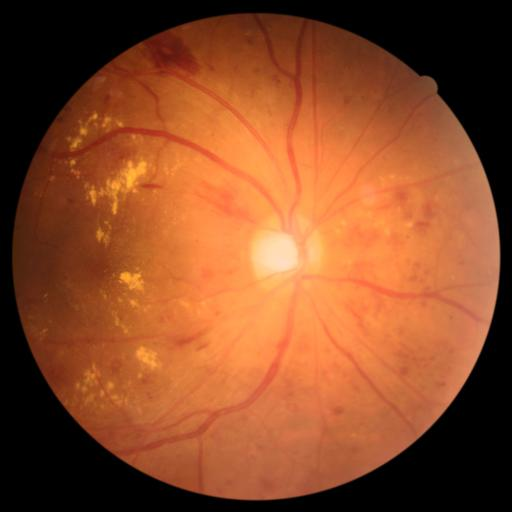
\includegraphics[width = 0.24\textwidth]{images/12_r1.jpg}
\label{fig_deg_1}}
\hfil
\subfloat[]{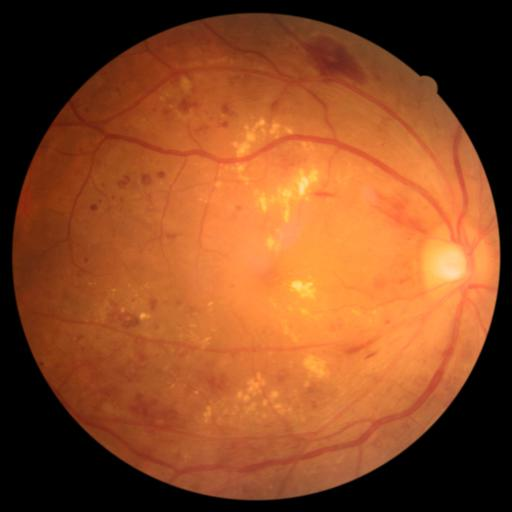
\includegraphics[width = 0.24\textwidth]{images/12_r2.jpg}
\label{fig_deg_2}}
\hfil
\subfloat[]{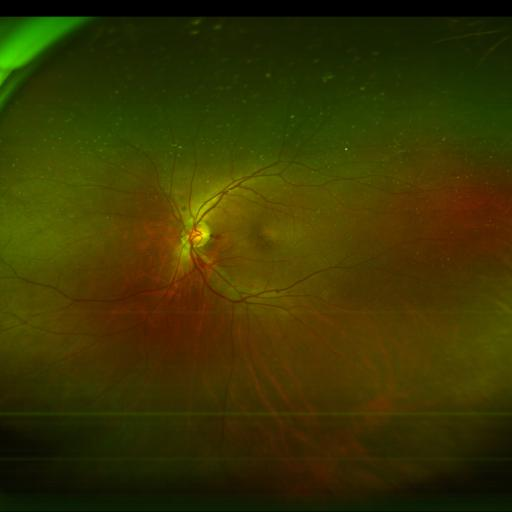
\includegraphics[width = 0.24\textwidth]{images/18_l2.jpg}
\label{fig_deg_3}}
\hfil
\subfloat[]{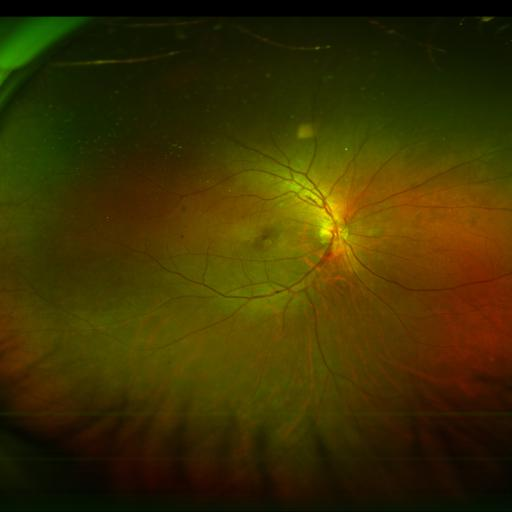
\includegraphics[width = 0.24\textwidth]{images/18_r1.jpg}
\label{fig_deg_4}}
\caption{Different image modalities involved in this challenge: (a) Optic Disc-centered retinal fundus image, (b) Macula-centered retinal fundus image, (c) Optic Disc-centered UW-Field retinal image, and (d) Macula-centered Ultra-Wild Field retinal image.}
\label{fig_samples}
\end{figure*}